% !TEX root = ../thesis.tex

\chapter{Solution} \label{solution}


Intertext is a platform based on a straightforward premise; it is a family of applications that can interpret IUIDL, an XML based UI description language, and generate appropriate front-ends for the host platform on the fly. Simply put, a developer wanting to create a front-end application uses a generic backend to generate IUIDL, and serve it from an endpoint, say at https://intertext.example.com. Users who wish to use this application uses an Intertext client on their preferred device or environment and visit this domain just like in a web browser. The Intertext client then makes a request to this domain, fetches the IUIDL served by this endpoint and generates the user interface as per the instructions received via IUIDL. (Fig ~\ref{fig:how_intertext_works})


Rather than rendering a simple static view, it performs some tasks such as accepting user input, navigating to different screens, making additional requests to fetch more data, keeping the UI updated and reading and writing some data to users local storage; all of which is again orchestrated based on the instructions received by the backend in IUIDL syntax.


\begin{figure}
  \centering
  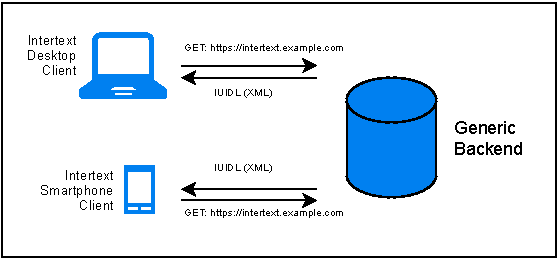
\includegraphics[width=13cm]{thesis/paper/images/how_it_works.pdf}
  \caption{A diagram showing the general workings of Intertext}%
  \label{fig:how_intertext_works}%
\end{figure}


Intertext aims to support multiple software clients (at the time of this paper, web and command-line interface clients are implemented, with more on the way) built natively for various platforms that can interpret IUIDL most appropriately to the host device or platform. For instance, users browsing an Intertext app through a smartphone receives an experience optimized for touch screens, command-line interface client users receive an optimized experience for a text-based interface or a user browsing from a low-end device with limited capabilities use the version optimized for low-performance devices to get a comfortable viewing experience and so on. 

% !TEX root = ../../thesis.tex

\section{Design Principles} \label{designPrinciples}

In order to address the problems mentioned in the \nameref{problemStatement} (\ref{problemStatement}) section, we adopted and implemented the following design principles.

\subsection{No foreign code execution}

There is no foolproof way of entirely securing a piece of software; even the most mature platforms and operating systems sometimes end up vulnerable to security exploits. However, without the ability to execute code on a platform, it is not directly possible to take advantage of vulnerabilities, even when there is one. Furthermore, the nature of Intertext allowed us to adopt disallowing code execution as a design principle. Intertext clients only accept UIUDL code, which is in XML and is not executable. Should a server send anything else, Intertext clients will simply ignore it. Thus, we can guarantee security for the users, regardless of the platform they are using the Intertext client on.

\subsection{Transparency}

Privacy is a common concern among users; primarily due to the recent scandals and data leaks, people started getting more conscious about their data. There is an increasing demand for users to be more in control and be aware of what is exposed and what is not. In order to address this burning need, we adopted transparency as a design principle. 

The most prominent way of achieving this is to have Intertext clients be in control of all interactions with the device and with external sources and keep logs in order to make them transparent to the user. The above-mentioned principle that no foreign code will be executed goes hand-in-hand in achieving this, as it would be unrealistic to expect complete control as it would be a non-deterministic approach. A good analogy would be to think of Intertext clients as an API endpoint that runs on users devices and exposes fundamental interactions with the host device and external networks through an API in a fully controlled manner. An application could "instruct" the Intertext client via IUIDL to perform some actions, such as making a network request, storing data, and accessing the local storage. Intertext client will then block this action until the user grant permission and keep logs every time before performing an action (Fig \ref{fig:permission_flow})

\begin{figure}
  \centering
  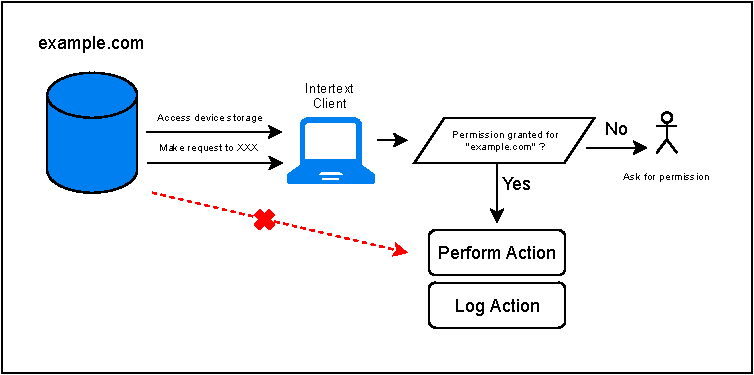
\includegraphics[width=13cm]{thesis/paper/images/permission.pdf}
  \caption{A diagram showing the permission flow}%
  \label{fig:permission_flow}%
\end{figure}


\subsection{Black-box Components as Building Blocks}

Intertext adopts a component based approach, we provide a set of components for developers to use to build their applications with. Each component accepts a set of properties, which gives them certain functionality or appearance. Developers are to use these components through IUIDL. For example, the IUIDL code below (at Figure \ref{fig:iuidl_buttons}) and it's output for Intertext web version (at Figure \ref{fig:iuidl_buttons_output}) shows some of the properties that \textit{button} component accepts. Layout properties such as  \textit{marginButton} allows positioning of the buttons to be customised, \textit{intent} properties gives the button a different look based on the use-case, properties like \textit{disabled} can alter its behaviour and so on.

\begin{figure}
\begin{minipage}{\linewidth}
\begin{lstlisting}[language=html]
<h3>Buttons</h3>

<grid cols="[1,1]">
  <block>
    <button marginBottom="2">default</button>
    <button marginBottom="2" disabled="true">disabled</button>
  </block>
  <block>
    <button marginBottom="2" intent="default">default</button>
    <button marginBottom="2" intent="primary">primary</button>
    <button marginBottom="2" intent="error">error</button>
    <button marginBottom="2" intent="warning">warning</button>
    <button marginBottom="2" intent="success">success</button>
    <button marginBottom="2" intent="info">info</button>
  </block>
</grid>
\end{lstlisting}
\end{minipage}
\caption{UIUDL that renders buttons in several states}%
\label{fig:iuidl_buttons}%
\end{figure}

\begin{figure}
  \centering
  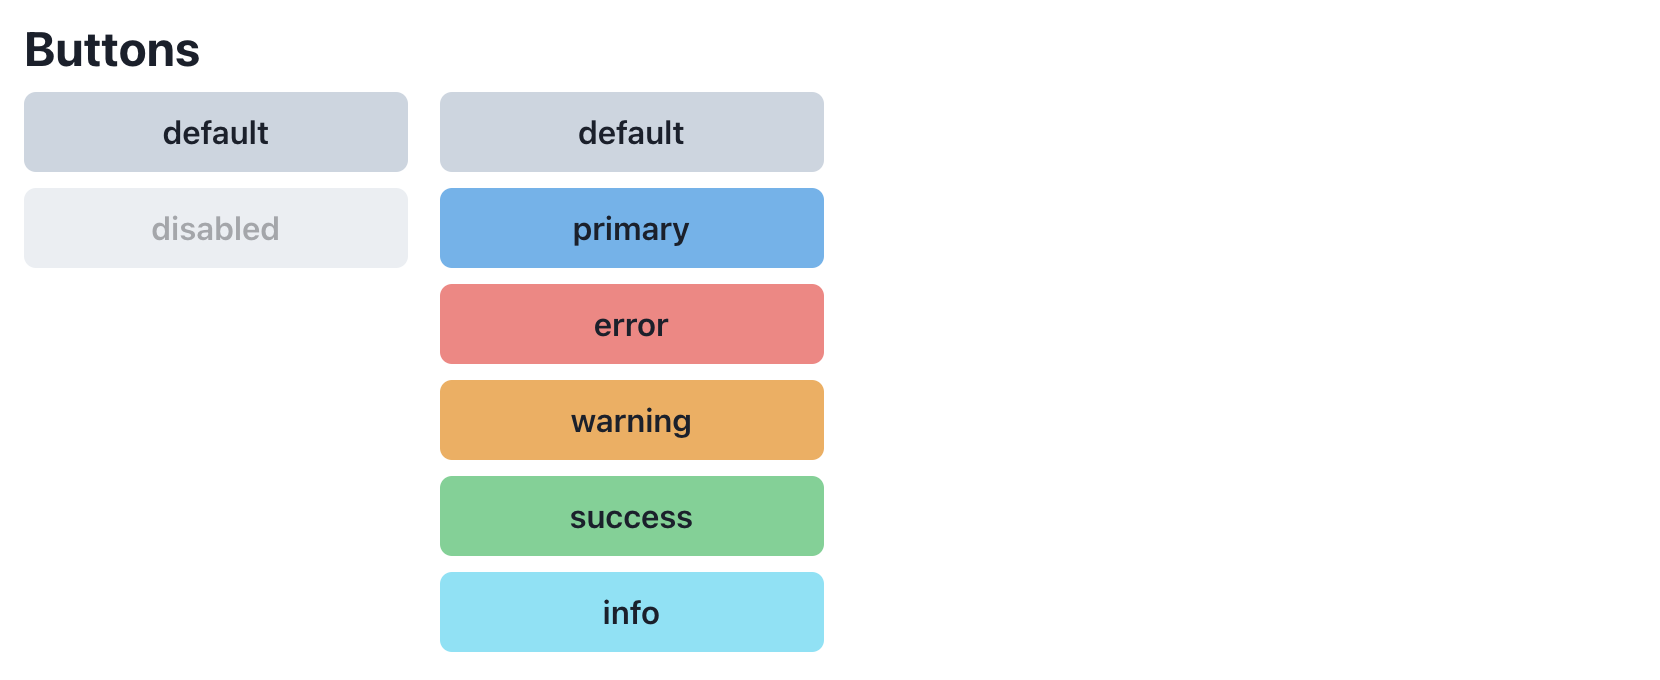
\includegraphics{thesis/paper/images/buttons.png}
  \caption{Output of IUIDL at Figure \ref{fig:iuidl_buttons} on Intertext web client}%
  \label{fig:iuidl_buttons_output}%
\end{figure}

However other than properties that components accepts, they cannot be modified or altered by the developer. The main motive behind this principle is standardisation. When all Intertext applications uses the same set of components, we can control how they look and how they are implemented, and ensure certain behavioural and visual aspects to bring the benefits in order to solve some of the problems mentioned in the \nameref{problemStatement} section.

Consistency is one of the most important benefit that this principle enables. A standard look and feel for components helps users to never get disoriented across applications, and recognise similar patterns easily. Another benefit is customisability, it is only possible to create one-size-fits-all themes that applies to every component in every application when all the applications uses components that are built in the same way. Another thing that comes to mind is accessibility. We established in section \ref{problemStatement} that accessibility is a big issue that not all developers choose to address. This principle allows us to take this responsibility from the developers hands by providing accessible components as building blocks. 

\begin{figure}[H]
  \centering
  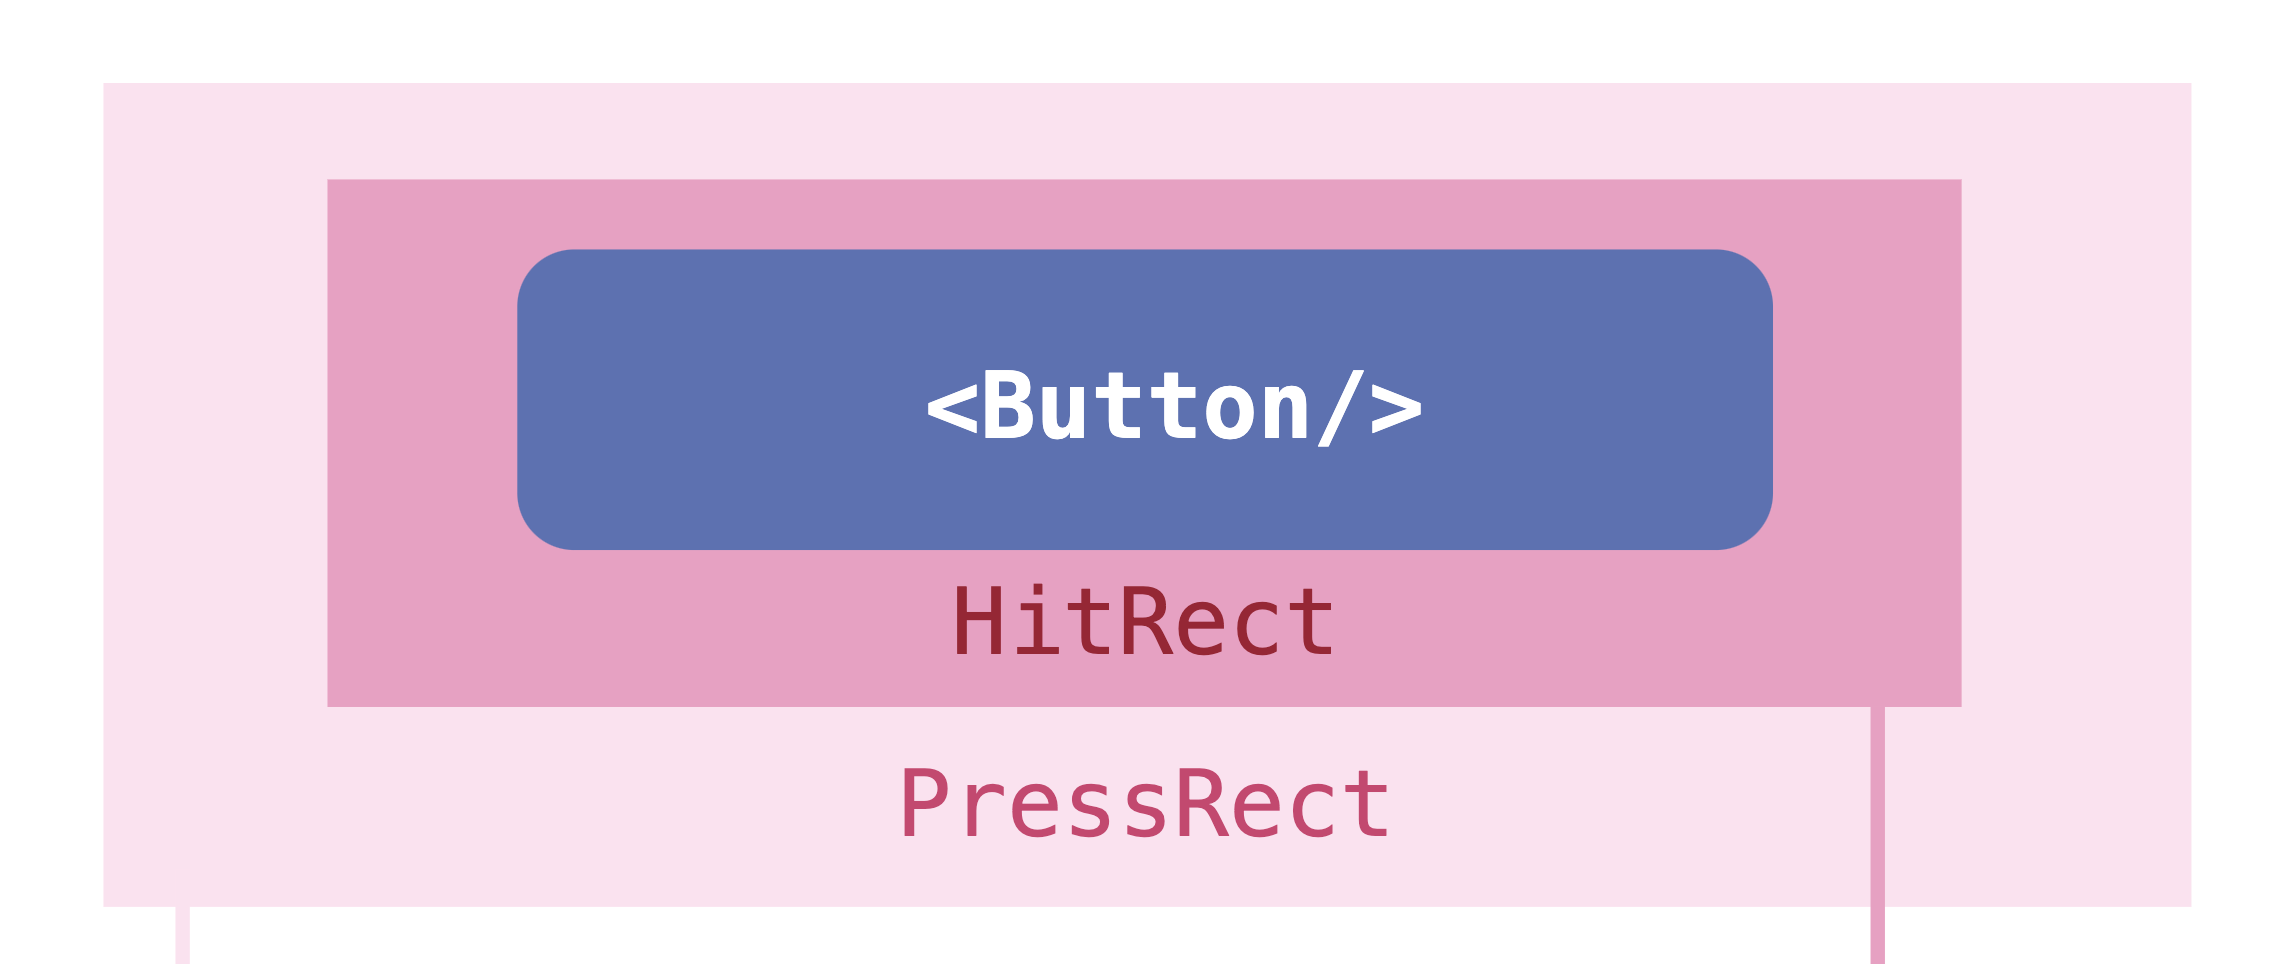
\includegraphics[width=13cm]{thesis/paper/images/pressable.png}
  \caption{Diagram that shows the implementation of Pressable component in React Native (reactnative.dev/docs/pressable)}%
  \label{fig:pressable}%
\end{figure}

Last but not least, this principle was crucial to achieve cross-device compatibility. The appearance and behaviour of components differs between implementations of the Intertext clients. For instance, the \textit{button} component on the web version needs not to be too big as clicks are precise, it requires a hover and focus state and so on. For a touch interface however, it needs to be bigger, and handle the caveat of having less precision by accepting hits on an area around it as seen in figure \ref{fig:pressable}. Every feature that components have needs to be supported as much as possible on different platforms that has different requirements. Having components with a fixed set of features allowed us to implement them all for different Intertext clients.

\subsection{Shared syntax between clients}

We designed IUIDL to be a generic markup language, agnostic of any platform or interaction type, and be based purely on XML so it could be consumed by all clients. This approach has many advantages, both for developers and users. It allows developers to create universal applications; once they start serving an Intertext application through an endpoint, any Intertext endpoint can consume the application through that endpoint. Moreover, it helps create a continual experience for the user; given that there is a shared layout system, UI elements will look and feel the same between Intertext clients. Figure \hl{TODO} and \hl{TODO} shows the similarities between Intertext web client and the command-line client.

\hl{TODO Add screenshots that shows similarities between the web version and the cli version}

Also, this approach allows existing Intertext applications to adopt to new Intertext clients as they are built in the future. At the time of this paper, Intertext web client and command-line client is ready, but as mentioned in the \hl{TODO: Future Work} section, more Intertext clients are on the way. Thanks to this principle, Intertext clients will have immediate availability for the upcoming Intertext clients.

% !TEX root = ../../thesis.tex

\section{Intertext UIDL} \label{intertextUIDL}
% !TEX root = ../../thesis.tex

\section{Intertext Clients} \label{intertextClients}

Intertext clients are the user facing products of Intertext, that build the bridge between the user and servers that serve IUIDL. They are meant to be implemented natively for the host platform in the most optimal way possible. 

For example, on mobile platforms such as iOS and Andriod, UI elements would be larger and more suitable for touch interactions. Primary interaction would be translated as \texttt{tap} while secondary interactions, if any, would be translated as \texttt{tap and hold}. The layout would adjust itself based on the screen size. The client would be implemented with either native technologies such as Swift/Objective-C for iOS and Kotlin/Java for Android, or with hybrid technologies that gets compiled into native code, such as React Native or Flutter for maximum responsiveness and efficiency. 

At the time of this paper, a web client and a command-line client is implemented. Native clients for iOS and Android, and desktop clients for Mac OS, Windows and several Linux distributions are among the ones that are planned, more could be found in \nameref{futureWork} section.

Intertext clients consists of two main parts; components and commands. Each Intertext client implement these separately, based on the host platform and its capabilities. Each client also implements the  their own local storage, state management strategy, and communication technique with the server.

\subsection{Components}

Components are anything that has a visual representation. All component stem from a generic IUIDL definition, and is interpreted based on the host platform requirements. They can be organisational or presentational. Organisational components are the layout components, they are used to position presentational components on the screen. Intertext implements a version of css flexbox specification as a layout system, which could be used to implement responsive interfaces for all screen sizes. For non browser-based platforms, we use the popular Yoga layout engine, which is a standalone implementation of the css flexbox specification in C++, allowing us to target almost any platform. More details on the layout system is given in \nameref{implementation} section.

Most presentational Intertext components share a concept, "intent", which is a way to communicate the intention of the UI element based on its use-case. Intertext clients renders the UI elements differently based on its intent, allowing a way for the developer to convey an intention of an UI element to the user without being able to intercept with the styles. For instance, an error message could be shown in a block component that has the intent "error", and it will be rendered with a red background, indicating to the user that it is an error message. Figure \ref{fig:intents} shows an example of intents on block component for Intertext web client.

\begin{figure}
  \centering
  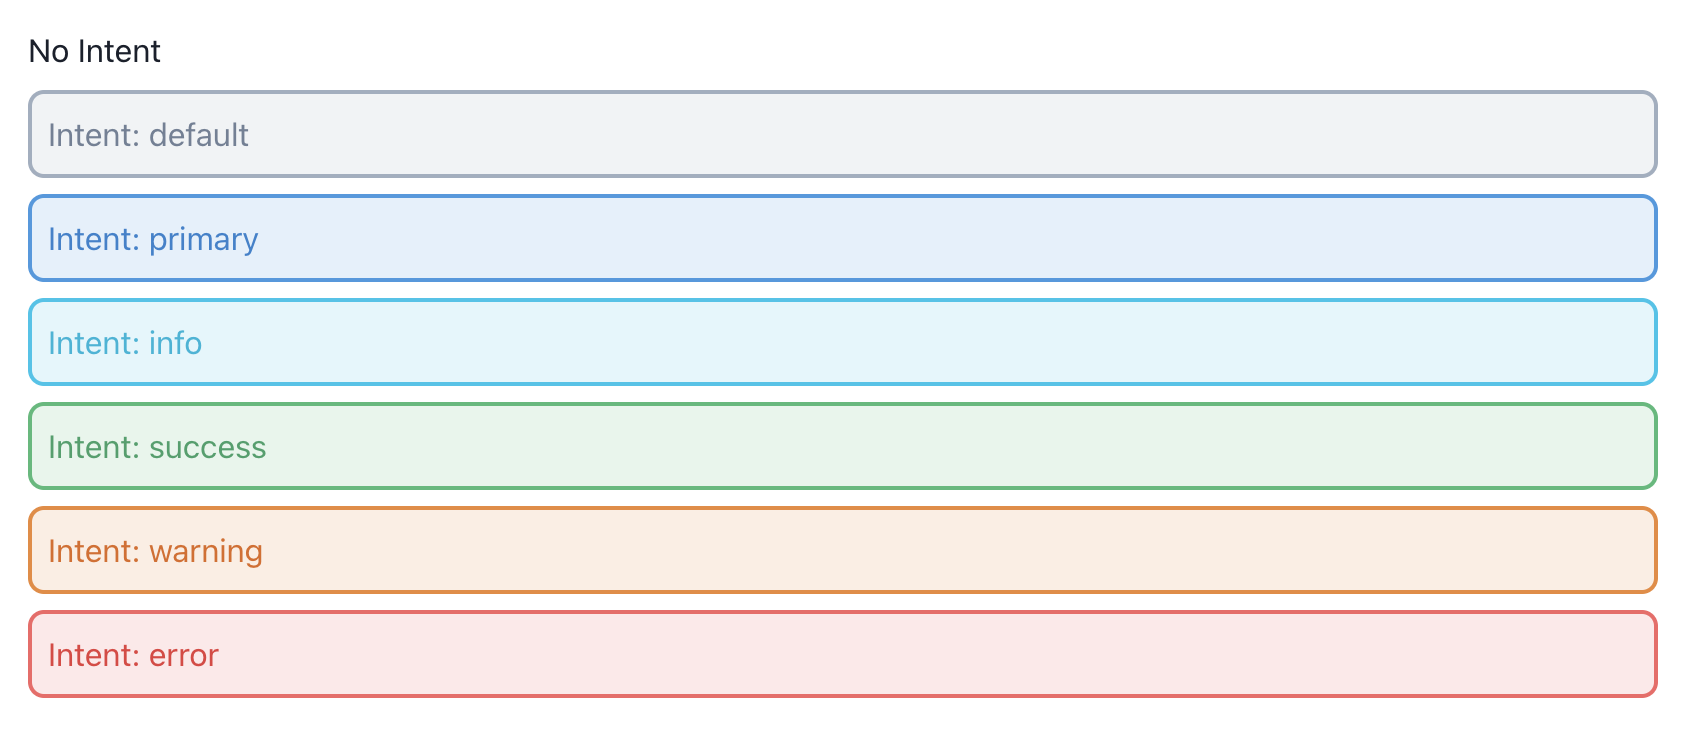
\includegraphics[width=13cm]{thesis/paper/images/intents.png}
  \caption{Intents for Block components}%
  \label{fig:intents}%
\end{figure}

\subsection{Commands}

Commands are IUIDL statements that are used to instruct Intertext clients to take an action. These actions can be triggered upon interaction with some components (such as clicking a button or submitting a form), a life-cycle event, with a timeout, or on page load. Commands are very primitive by design, they are not meant to build application logic with. They are merely for asking the Intertext client to communicate with the server, store something, read something that is stored, or retrieve some user data. Command system is designed in order to ensure Intertext client is aware of what it is being asked to do, so that it can control and restrict the entire flow, ask for permission from the user when necessary, or simply refuse to take an action if needed. 

Figure \ref{fig:ex_cmd_post_timeout} shows an example of how a network request action can be executed upon a delay, and Figure \ref{fig:ex_cmd_form} shows how a form can be submitted with reference to input fields. More on commands will be on \nameref{implementation} section.

\begin{figure}
\begin{minipage}{\linewidth}
\begin{lstlisting}[language=xml]
<timeout delay="1000">
  <request endpoint="/refresh"></request>
</timeout>
\end{lstlisting}
\end{minipage}
\caption{Post command on Timeout}%
\label{fig:ex_cmd_post_timeout}%
\end{figure}

\begin{figure}
\begin{minipage}{\linewidth}
\begin{lstlisting}[language=xml]
<input name="item_title"></input>
<input name="item_description"></input>
<button>
  <text>Submit</text>
  <button.onClick>
    <request endpoint="/items/save"></request>
  </button.onClick>
</button>
\end{lstlisting}
\end{minipage}
\caption{Form command with reference on server side to internal input values}%
\label{fig:ex_cmd_form}%
\end{figure}

\begin{figure}
\begin{minipage}{\linewidth}
\begin{lstlisting}[language=javascript]
router.get('/signup', async (req, res, next) => {
  
  const currentStep = req.body.state?.current_step ?? 0
  const currentInputState = req.body.inputState
  const previousInputState = req.body.state.input_state
  
  // check if user finished the form
  if (currentStep == LAST_STEP) {
    
    // execute signup logic
    const error = await signupUser(req.body.state?)
    
    // render success or error page based on
    // the signup result
    res.render(error
      ? 'signup_form_error'
      : 'signup_form_success',
    { error });
  
  } else {
    
    // render signup form
    res.render('signup_form', {
      // increment the current step
      step: currentStep + 1
      // merge current form data with previous
      inputState: merge(
        previousInputState,
        currentInputState
      )
    });
  }
});
\end{lstlisting}
\end{minipage}
\caption{Handling a sign-up flow with multiple steps}%
\label{fig:state_signup_progress_js}%
\end{figure}

\subsection{State Management}

Intertext clients offer basic state management, making it possible to serve stateful Intertext applications using serverless/stateless backends. Front-end state can be fully driven from the backend via IUIDL. Intertext client offers two types of storage, persisted and volatile. 

Volatile storage is kept in the memory and it is persisted across the session. The purpose of this storage is to keep temporary values, such as users' progress in a long form distributed across multiple pages. Intertext clients passes the entire application state on the volatile storage to the backend on every request, allowing backend to build logic around the current state of the front-end application, and serve the UI accordingly. Figure \ref{fig:state_signup_progress_js} and Figure \ref{fig:state_signup_progress_xml} show this through an hypothetical sign up form with steps distributed across multiple steps. Figure \ref{fig:state_signup_progress_js}, we see the pseudo-code implementation of the stateless backend for this scenario. It can be seen that the current step user is at, and the input state data collected thus far is kept in the volatile state on the front-end. The state gets passed on to the backend on every request made to the \texttt{/signup} endpoint. We retrieve the current step, and serve different responses accordingly. If user completed the last step, then we execute our application logic (which in this case is signing user up), and render the result page. Otherwise, we increment the current step, combine the form data collected thus far, and render the form template with these. On the form template in Figure \ref{fig:state_signup_progress_xml}, we use the \texttt{<state>} block to instruct the Intertext client to record these new set of data to the front-end, so it could be passed on to the backend on the next request. Moreover, we render the correct form UI based on the step user is currently at.

Another type of storage is the persisted storage. As the name suggests, values stored this way is persisted across sessions. Unlike the volatile storage, in which the data is kept in the memory, persisted storage gets stored locally using the storage option available to the host platform. By default, data available in the persisted storage is not passed on to the backend in every request automatically, but can be configured to do so.

In order to protect user privacy, Intertext clients block cross-origin storage reads/writes, preventing users to be tracked across Intertext applications. In another words, state management is bound to the origin. Lets say \texttt{sub1.example.com} wrote data to the storage. This data can only be read or manipulated by the very same domain. \texttt{sub2.example.com} or \newline\texttt{sub.example2.com} or any other domain will not have access to this data. While this behaviour protects users from cross-origin tracking, it may also inconvenience some users, especially in scenarios such as services that shares the same user login that is distributed across multiple domains/subdomains. As mentioned further in the \nameref{futureWork} section, we plan to add a feature where Intertext clients would ask for user permission to share data between domains/subdomains instead of directly blocking it.

\begin{figure}
\begin{minipage}{\linewidth}
\begin{lstlisting}[language=xml]
<!-- signup_form -->

<!-- set front-end state to read on later requests  -->
<state key="current_step">{{ step }}</state>
<state key="input_state">{{ inputState }}</state>

{{#ifEquals step 1}}
  <!-- form elements for step 1 -->
{{/ifEquals}}

{{#ifEquals step 2}}
  <!-- form elements for step 2 -->
{{/ifEquals}}

<!-- ... -->
\end{lstlisting}

\begin{lstlisting}[language=xml]
<!-- signup_form_success -->

<h1 intent="success">Sign Up Successful!</h1>
<p intent="success">Please check your verification email</p>
\end{lstlisting}

\begin{lstlisting}[language=xml]
<!-- signup_form_error -->

<h1 intent="error">Something went wrong</h1>
<p intent="error">{{error}}</p>
\end{lstlisting}

\end{minipage}
\caption{Template files for multi-step sign up flow at Figure \ref{fig:state_signup_progress_js}}%
\label{fig:state_signup_progress_xml}%
\end{figure}

% !TEX root = ../../thesis.tex

\section{Communication} \label{communication}


% - How it addresses problems
% - Describe theoretically (not too much details)
% - Client, Server etc.
% - Technical-ish / Conceptual / Architecture 



% - design principles
%   - no foreign code executions / only data
%   - no foreign styling / customisable styles
%   - transparency
%     - all front-end ops goes through intertext client (requests from the server)
%     - all requests goes through intertext client (youtube embed etc.)
%   - all platforms shares the same syntax
  

% - intertext uidl
%   - terminologies? (platform-specific etc.)
%   - limitations?
%   - json? xml?
 
% - clients
%   - server-side rendering
%   - engine
%   - state
%   - layout
  
% - communication
%   - ui manipulation technique
%     - front-end manipulation
%     - backend manipulation
%   - front-end state management